

The hardware consists of network cameras connected directly by Ethernet to a processing unit. The system should be able to handle cameras with a resolution of at least 2M pixel. Cameras are running on PoE, power over Ethernet, which enables easier installment. 
The processing unit is a server which uploads the calculated results to a web service. 

\begin{figure}[htb]
	\centering
	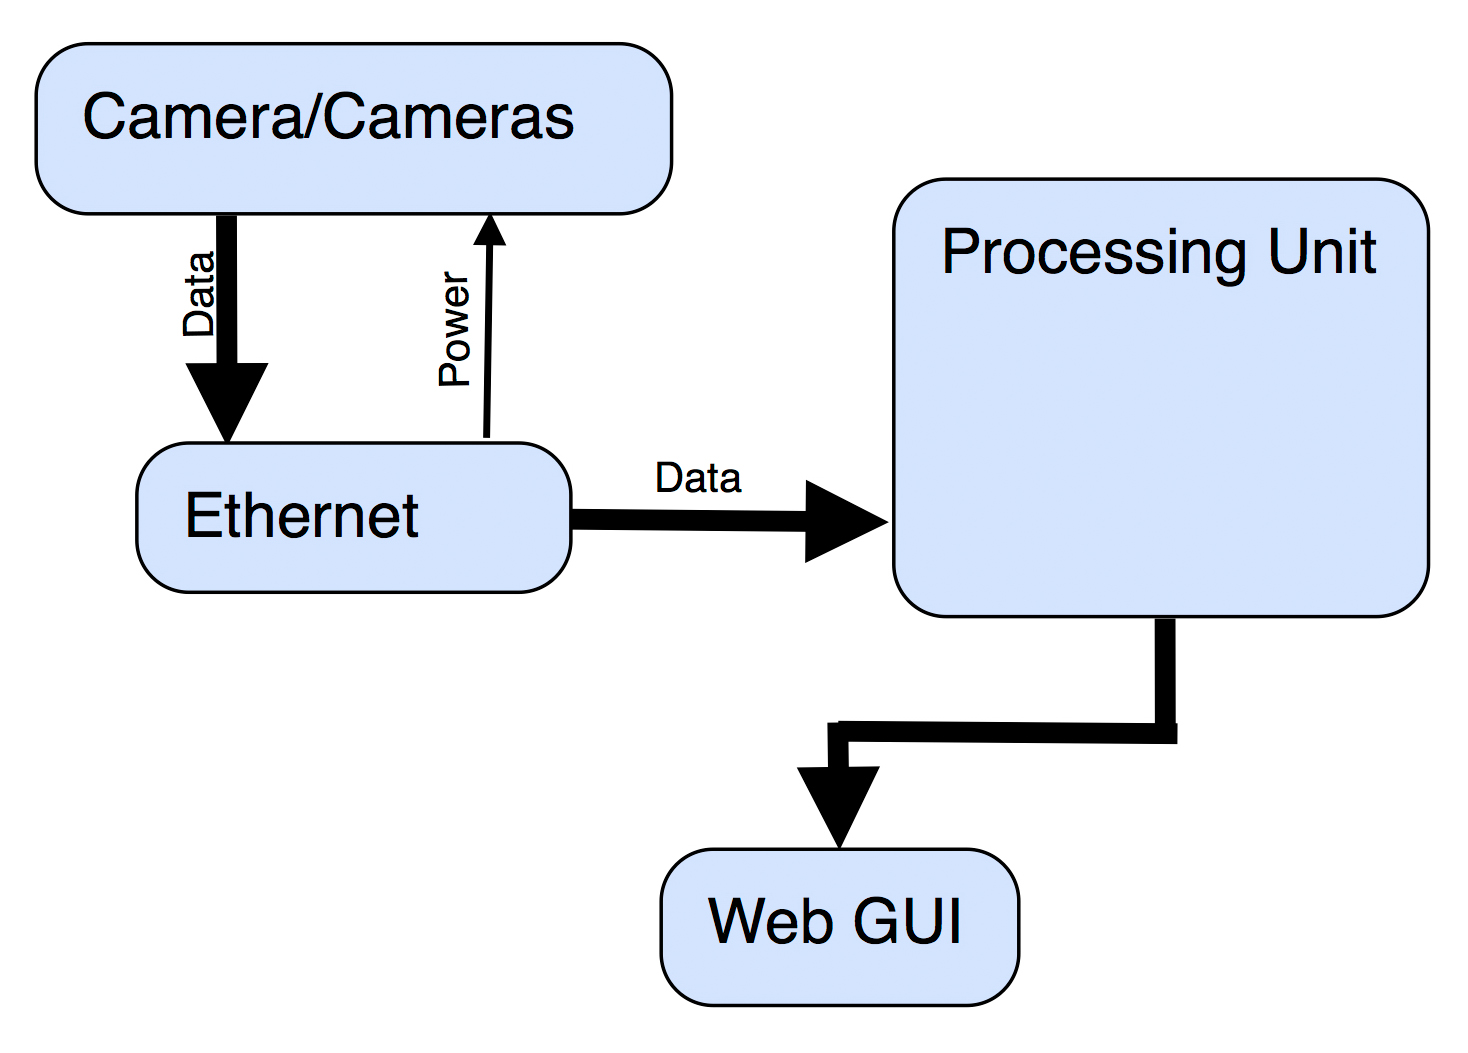
\includegraphics[width=160mm]{images/Hardware-flowchart.jpg}
	\caption[This text ends up at the list of figures]{\textit{Flowchart harware modules}}
	\label{fig:block_overview_fig}  %Skapar referens till figuren
\end{figure}


\subsection{Limitations}
The hardware is limited by budget, internet connection and the source of power. The cost is limited to approximately 15.000 SEK per room, including installation costs. The budget limits performance of the cameras e.g. resolution and number of cameras. Cameras use power over Ethernet, which limits their maximal power usage to around 15-25 W, depending on the present Ethernet standard. Powering cameras with normal wall sockets can be expensive if it requires installing new wall sockets, therefore source of power is a limitation. The Ethernet connection needs to be stable and have a bandwidth good enought for sending live video from the cameras.   

\subsection{Hardware Requirements}
\label{sec:hardware_req}
\reqtable
{
	\addreq{The system uses network cameras powered via Ethernet}{1}	
	\addreq{The system can operate using high resolution ($>$2 Mpixel) cameras}{1}
	\addreq{Lower resolution cameras can be used}{2}
	\addreq{The application can run using the processing power provided by the costumer}{1}
	\addreq{The application can run using a mid-end processing device}{2}
	\addreq{The application can run using a low-end processing device}{3}
}